\documentclass{beamer}

\usetheme{MagdeburgFIN}
\usefonttheme{structurebold}
\usepackage{graphicx}
\usepackage{float}
\usepackage{url}
\usepackage{pdfpages}
\usepackage[export]{adjustbox}
\usepackage{wrapfig}
\usepackage{verbatim}

\setbeamertemplate{caption}[numbered]

\title{Build Your Own OctopusDB: Blinktopus Edition}
\author{Ali Hashaam, Ali Memon, Guzel Mussilova, Pavlo Shevchenko}
\date{July 10, 2017}
\institute{Scientific Project: Databases for Multi-Dimensional Data, Genomics and Modern Hardware}

\begin{document}

\begin{frame}[plain]
 \titlepage
\end{frame}

\begin{frame}
\frametitle{Table of Contents}
\tableofcontents
\end{frame}

\section{Motivation/Problem Statement}
\begin{frame}
\frametitle{Motivation}
\begin{enumerate}
\item{Companies need to pick only specialized DBMSs, each tailored to their specific use-case. \\ \pause
$\Rightarrow$ Need for \emph{one size fits all system} (e.g. HTAP)}
\pause
\item{Support OLAP queries for analysis over real-time data (i.e., freshness). \\ \pause
$\Rightarrow$ Explore the techniques related to more interactive queries (e.g. \emph{Approximate Query Processing})}
\end{enumerate}
\end{frame}

\section{Background}
\begin{frame}
\frametitle{Background}
\begin{enumerate}
\item{\textbf{OctopusDB}} \pause
\begin{itemize}
\item{uses logs as a primary storage;} \pause
\item{mimicks several types of systems (OLAP, OLTP, etc.) by representing them as \emph{Storage Views}.}
\end{itemize}
\pause
\item{\textbf{BlinkDB}}
\begin{itemize}
\item{successfully integrates AQP techniques into its architecture.}
\end{itemize}
\end{enumerate}
\end{frame}

\section{Conceptual Idea and Implementation}
\begin{frame}
\frametitle{Conceptual Idea and Implementation}
\begin{figure}
\centering
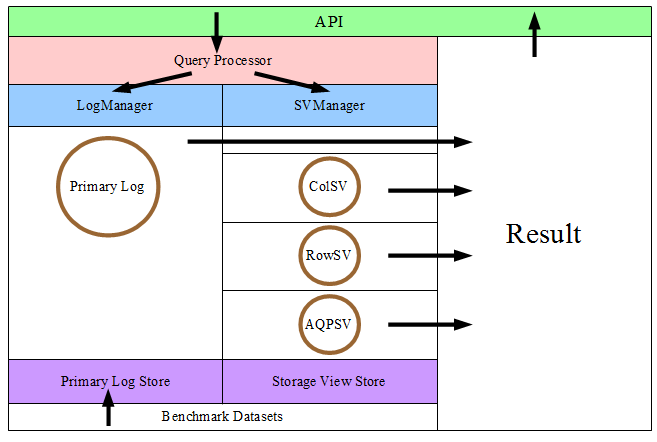
\includegraphics[scale=0.5]{img/blinktopus_architecture.png}
\caption{OctopusDB Architecture.}
\end{figure}
\end{frame}

\begin{frame}
\frametitle{Conceptual Idea and Implementation}
\textbf{Which synopses to pick?} \pause
\begin{itemize}
\item{Equi-depth histograms}
\begin{itemize}
\item{suitable for range queries;}
\item{simple to implement and interpret.}
\end{itemize}
\pause
\item{Sketches}
\begin{itemize}
\item{DISTINCT COUNT queries;}
\item{\emph{HyperLogLog};}
\item{\textit{DataSketches} library by \textit{Yahoo!} \footnote{https://datasketches.github.io}}
\end{itemize}
\end{itemize}
\end{frame}

\section{Evaluation Setup and Results}
\begin{frame}
\frametitle{Evaluation Setup} \pause
\textbf{Machine}
\begin{itemize}
\item{CentOS Linux 7.1.1503}
\item{Java SDK 8u131-b11-linux-x64}
\item{2 Intel(r) Xeon (TM) E5-2630 v3s CPU @ 3.2GHz processors (8 cores each) and 1024 GiB memory}
\end{itemize}
\pause
\textbf{Benchmark Datasets}
\begin{itemize}
\item{TPC-H datasets (Orders and Lineitems)}
\end{itemize}
\pause
\textbf{Experiments}
\begin{enumerate}
\item{Average response time for a range query on the Orders table with various scaling factors and predicate selectivity.}
\item{Average response time for a count-range query on the Orders table. Comparison with an equi-depth histogram.}
\item{Average response time for a count distinct query on the Orders table. Comparison with a HLL sketch.}
\end{enumerate}
\end{frame}

\begin{frame}
\frametitle{Results. Experiment 1}
\centering
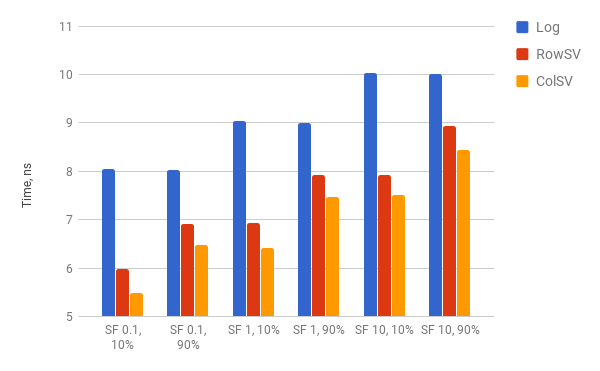
\includegraphics[scale=0.5]{img/exp1.png}
\end{frame}

\begin{frame}
\frametitle{Results. Experiment 2}
\centering
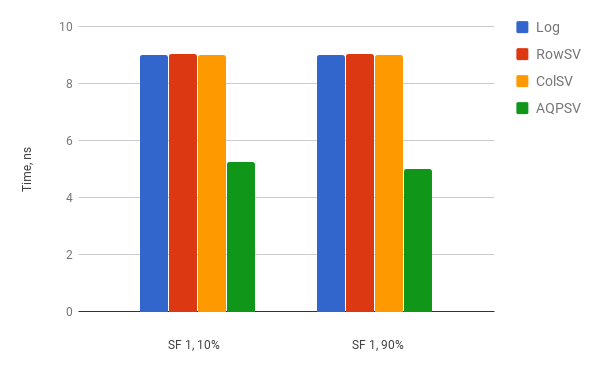
\includegraphics[scale=0.5]{img/exp2.png}
\end{frame}

\begin{frame}
\frametitle{Results. Experiment 3}
\centering
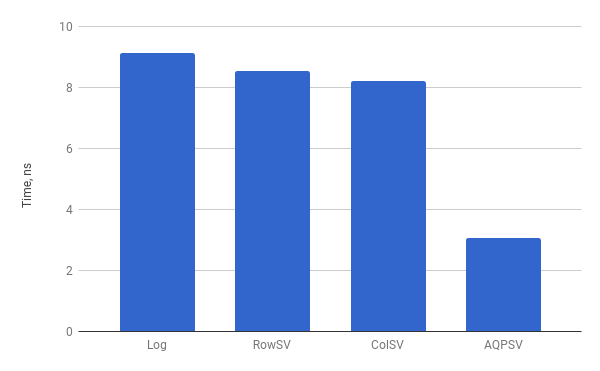
\includegraphics[scale=0.5]{img/exp3.png}
\end{frame}

\begin{frame}
\frametitle{Challenges} \pause
\centering
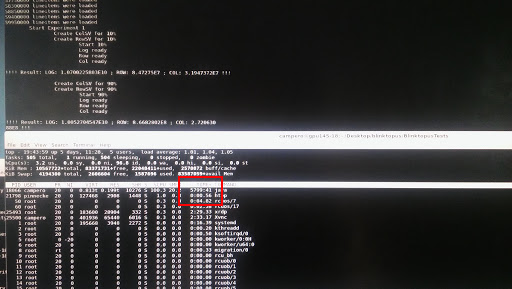
\includegraphics[scale=0.5]{img/beast.jpg} \\ \pause
10900 min = 182 hours = 7.5 days
\end{frame}

\section{Related Work}
\begin{frame}
\frametitle{Related Work} \pause
\begin{enumerate}
\item{\textbf{Apache Samza}}
\begin{itemize}
\item{logs as a primary storage;}
\item{replicates logs on multiple nodes.}
\end{itemize}
\pause
\item{\textbf{Rodent Store}}
\begin{itemize}
\item{represents data in the various physical layouts;}
\item{provides DBAs a high-level interface to specify the data physical representation by means of storage algebra.}
\end{itemize}
\pause
\item{\textbf{Snappy Data}}
\begin{itemize}
\item{AQP Support;}
\item{uses numerous types of synopses (samples, sketches);}
\item{user defines the level of accuracy and the number of column sets to approximate the results.}
\end{itemize}
\end{enumerate}
\end{frame}

\section{Conclusion and Future Work}
\begin{frame}
\frametitle{Conclusion} \pause
\begin{itemize}
\item{Systems with adaptive layouts can be effectively combined with AQP techniques.} \pause
\item{OLAP queries can benefit from AQP techniques.} \pause
\item{Non-optimized central log as a primary storage is quite prohibitive.}
\end{itemize}
\end{frame}

\begin{frame}
\frametitle{Future Work}
\begin{itemize}
\item{optimize centralized log (e.g. log replication, garbage collection);} \pause
\item{evaluate the efficiency of the concurrency control scheme of OctopusDB;} \pause
\item{evaluate the memory footprint of histograms and sketches;} \pause
\item{extend Blinktopus architecture to support transactional model;} \pause
\item{extend query classes by implementing sample-based data synopses.}
\end{itemize}
\end{frame}

\section{Demonstration}
\begin{frame}
\frametitle{Demonstration}
\begin{figure}
\centering

\includegraphics[scale=0.1]{img/wink.png}

\includegraphics[scale=0.1]{img/oct_emoji.png}
\end{figure}
\end{frame}

\begin{frame}
\frametitle{Thank you!}
\end{frame}

\begin{frame}
 \frametitle{Questions? Recommendations? Remarks?}
\end{frame}

\end{document}
